\section{Overview of the results}\label{sec:overview}

\paragraph{Counts.}
\Cref{tab:classes} gives the classification of the 3{,}662 formats for which we hold a verified scheme. Of these, 795 are records: 733 below every listed rank in any ring, and 62 below every listed GF(2)-valid rank while another table lists an equal or lower rank for an unspecified or different field.
\begin{table}[t]
\centering\small
\begin{tabular}{@{}lr@{}}
\toprule
class of the best verified scheme of a sorted format & formats\\
\midrule
\textsf{below\_all}: below every listed rank in any ring & \textbf{733}\\
\textsf{gf2\_valid\_only}: below every listed GF(2)-valid rank only & \textbf{62}\\
\textsf{tie}: equal to the best listed rank & 1{,}413\\
\textsf{above}: above the best listed rank & 1{,}454\\
\midrule
formats with a verified scheme (of 5{,}456) & 3{,}662\\
\bottomrule
\end{tabular}
\caption{Classification of the scoreboard of 2026-09-29 against the four tables of \cref{tab:sources}.}
\label{tab:classes}
\end{table}

\paragraph{Where the records are.}
Records are overwhelmingly formats with a large side (\cref{tab:size,fig:maxside}): 734 of the 795 (92.3\%) have a side above 16 and 61 have all sides at most 16; only 9 have all sides at most 12 and 2 at most 8.
The share of verified formats that are records is 2--4\% for maximum side up to 12, 13\% for 13--16, and 24.6\% above 16.
\begin{table}[t]
\centering\small
\begin{tabular}{@{}lrrrrrr@{}}
\toprule
largest side & \textsf{below\_all} & \textsf{gf2\_valid\_only} & records & verified formats & universe & records/verified\\
\midrule
2--8 & 2 & 0 & 2 & 84 & 84 & 2.4\%\\
9--12 & 5 & 2 & 7 & 202 & 202 & 3.5\%\\
13--16 & 34 & 18 & 52 & 394 & 394 & 13.2\%\\
17--24 & 263 & 15 & 278 & 1{,}129 & 1{,}620 & 24.6\%\\
25--32 & 429 & 27 & 456 & 1{,}853 & 3{,}156 & 24.6\%\\
\midrule
all & 733 & 62 & 795 & 3{,}662 & 5{,}456 & 21.7\%\\
\bottomrule
\end{tabular}
\caption{Records by largest side. Every format with all sides at most 16 has a verified scheme; above 16 we hold schemes for 70\% and 59\% of the formats.}
\label{tab:size}
\end{table}

\begin{figure}[t]
\centering
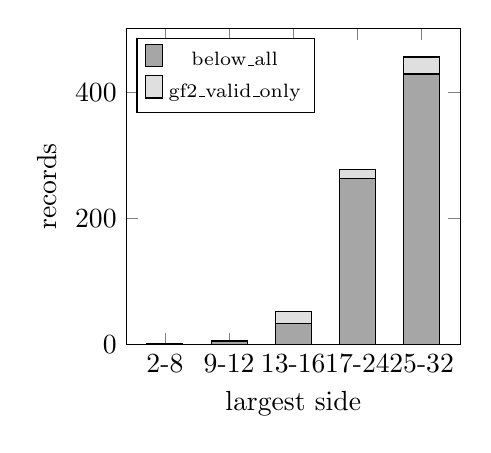
\begin{tikzpicture}
\begin{axis}[ybar stacked,width=0.48\textwidth,height=5.6cm,bar width=13pt,ymin=0,
  symbolic x coords={2-8,9-12,13-16,17-24,25-32},xtick=data,xlabel={largest side},ylabel={records},
  legend style={at={(0.03,0.97)},anchor=north west,font=\scriptsize},enlarge x limits=0.15]
\addplot[fill=gray!70] coordinates {(2-8,2) (9-12,5) (13-16,34) (17-24,263) (25-32,429)};
\addplot[fill=gray!25] coordinates {(2-8,0) (9-12,2) (13-16,18) (17-24,15) (25-32,27)};
\legend{below\_all,gf2\_valid\_only}
\end{axis}
\end{tikzpicture}\hfill
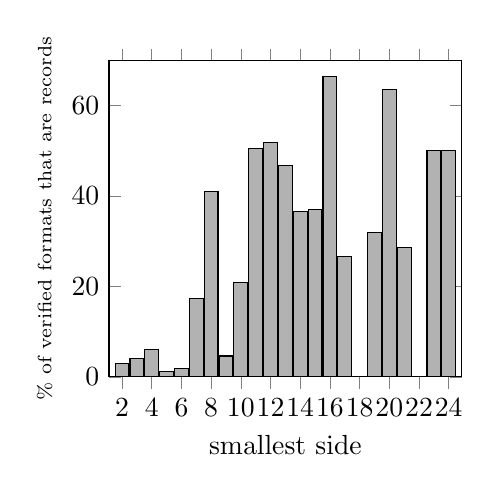
\begin{tikzpicture}
\begin{axis}[ybar,width=0.5\textwidth,height=5.6cm,bar width=5pt,ymin=0,ymax=70,
  xtick={2,4,6,8,10,12,14,16,18,20,22,24},xlabel={smallest side},ylabel={\% of verified formats that are records},
  ylabel style={font=\scriptsize},enlarge x limits=0.04]
\addplot[fill=gray!60] coordinates {(2,3.0) (3,4.0) (4,6.0) (5,1.1) (6,1.8) (7,17.4) (8,40.9) (9,4.6) (10,20.9) (11,50.5) (12,51.8) (13,46.8) (14,36.6) (15,37.1) (16,66.4) (17,26.7) (18,0) (19,32.0) (20,63.5) (21,28.6) (22,0) (23,50.0) (24,50.0)};
\end{axis}
\end{tikzpicture}
\caption{Left: records by largest side. Right: the share of verified formats that are records, by smallest side (smallest sides 25--28 have 4--8 verified formats each, and none above 28).}
\label{fig:maxside}
\end{figure}

The right panel of \cref{fig:maxside} shows how the records depend on the smallest side: they are rare when it is between 2 and 6 (1--6\%), common between 11 and 16 (37--66\%), and irregular above 16 where few formats have been verified; there are dips at 9 (4.6\%) and 18 (none of 39 verified formats) and peaks at 8, 11--13, 16 and 20. We did not investigate the pattern; it is what one expects if improvements come from composing blocks of a few favourable sizes.

\paragraph{New and old.}
The scoreboard held 560 records on the morning of 2026-09-29 (533 \textsf{below\_all}, 27 \textsf{gf2\_valid\_only}) against the same tables. During the day 235 formats became records (200 and 35), 49 earlier records were lowered further (by 1{,}513 terms in total; median 22, at least 10 for 37 of them), and none was lost;
182 of the 235 new records are formats for which we had no verified scheme in the morning, and coverage of the universe rose from 31.2\% to 67.1\%.
Of the 560 earlier records, 189 descend from the July block-composition certificates, 140 from certificates committed 2026-09-22 to 09-26, 183 from closure products of the first days of the campaign, 40 from matmulcatalog replays, and 8 from public seeds and the project's live fleet; of the 235 new ones, 149 descend from closure products, 55 from replays and 31 from July or committed certificates.
